\documentclass[letterpaper,12pt]{article}
\usepackage[margin=1in]{geometry}
\usepackage{graphicx}  % Include figure files
\usepackage{xcolor}  % Allow for a color text
\usepackage{amsmath}  % math fonts
\usepackage{amsfonts}  % math fonts
\usepackage{latexsym}  % math fonts
\usepackage{amssymb}  % math fonts
\usepackage{mathtools} % Give more control of how equations are displayed
\usepackage{appendix} % Lets you create an appendix
\usepackage[numbered]{matlab-prettifier} % Let's me import MATLAB code in a nice format
\usepackage{indentfirst} % This indents the first paragraph. By default latex won't do it.

\newtagform{show_eq}{(Eq.\ }{)}  % how the equation numbers are displayed
\usetagform{show_eq} % this goes with the \newtagform

\begin{document}

% ================================== Title Page ==========================================
\begin{titlepage}
 \begin{center}
 \vspace*{1in}
{\Huge Comparison Between Experimental and Analytical Operational Amplifier in a Closed Loop Configuration Models}\\
    \bigskip
    by\\
    \bigskip
    {\Large Kevin Moran} \\
    \bigskip
    Lab Partner : Jorge\\
    Date of Experiment : Thursday, October 14th, 2020

    \bigskip\bigskip\bigskip
    University of Southern California\\
    Aerospace and Mechanical Engineering Department\\
    AME 341A : Mechoptronics
 \end{center}
\end{titlepage}


% ================================== Main Text ==========================================


% --------------------------------- Introduction ----------------------------------------------
\section{Introduction}
Operational Amplifiers, often referred to as \textit{op-amps}, are a vital part of data acquisition circuits and circuits that rely on threshold voltage inputs to activate additional components. As the name suggest, om-amps serve as voltage amplifiers and can be setup in various configurations using passive circuit elements such as resistors and capacitors. Figure \ref{NFL} illustrates a LM741 op-amp in a negative feedback loop configuration.

\begin{figure}[ht]
    \centering
    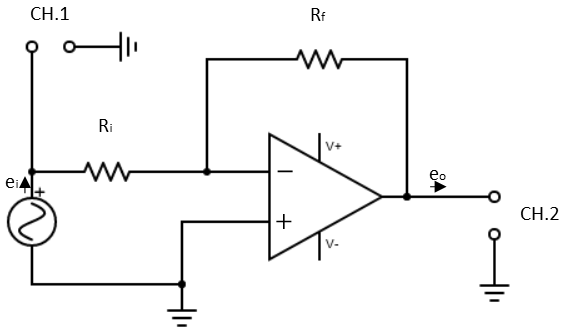
\includegraphics[scale=1.25]{feedback.png}
    \caption{\small LM741 operation amplifier negative feedback loop schematic. All components of the circuit are grounded using a common ground. CH1 and CH2 represent probe connection on Vbench Interface}
    \label{NFL}
\end{figure}

Other words


% -------------------------- Methods and Materials -------------------------------------------
\section{Methods and Materials}
This is where you write the methods and materials section


% --------------------------------- Results ----------------------------------------------
\section{Results}
This is where you show your results and key values

% --------------------------------- MATLAB ----------------------------------------------
\newpage
\appendix
\section{MATLAB Script}
\lstinputlisting[style=Matlab-editor]{lab6.m}

\end{document}